% !TeX spellcheck = en_US
\section{\sys Approach}
\label{sec_framework}

Based on the three key techniques in Section~\ref{sec_technique}, we develop a 
practical static approach named \sys, to detect data races in OS kernels, and 
estimate the harmfulness of these data races. We have implemented \sys with 
Clang~\cite{clang} and Z3~\cite{z3}. \sys can automatically mine locking rules, 
detects data races and estimates the harmfulness of detected data races. 
Figure~\ref{fig_architecture} shows the architecture of \sys, which has four 
phases:

\begin{figure}[htbp]
	\centering
	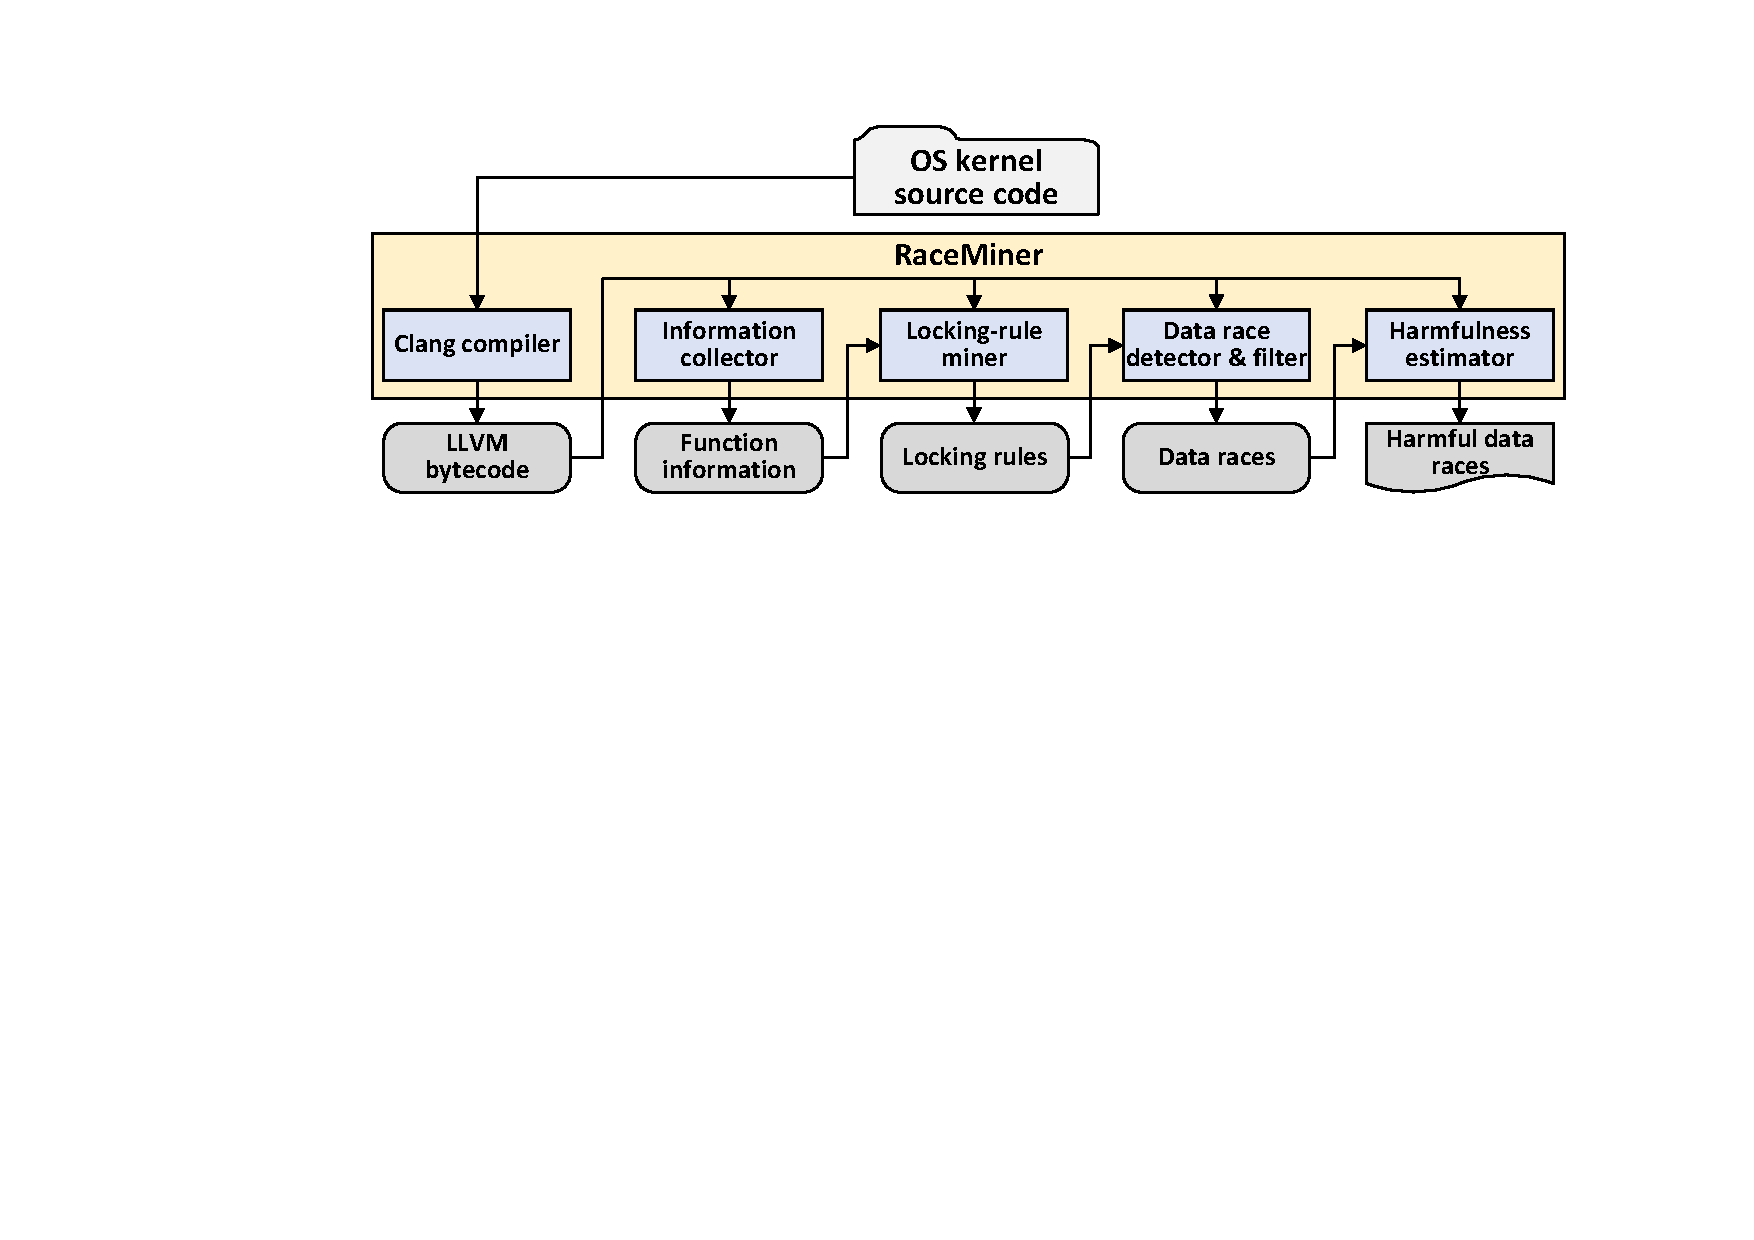
\includegraphics[width=1\linewidth]{figures/fig_architecture.pdf}
	\figcaption{\sys architecture.}
	\label{fig_architecture}
\end{figure}

\PP{P1: Source-code compilation.} The Clang compiler compiles the OS source 
code into LLVM bytecode, and then the information collector scans each LLVM 
bytecode file to record function information (including the position of each 
function definition and function name, etc.) in a database. Such information is 
used in subsequent code analysis for inter-procedural analysis across source 
files.

\PP{P2: Locking-rule Mining.} The locking-rule miner uses our alias-aware rule 
mining method to automatically deduce locking rules about whether accesses to a 
specific data structure field should be protected and which data structure 
field the protecting lock exist in

\PP{P3: Data race detection and false-positive filtering.} The data race 
detector detects data races by checking whether a given access violates the 
rules mined by our locking-rule miner. After finding a possible data race, the 
data race filter uses our locking-usage analysis to determine whether it is a 
false positive. Besides, for a given data race, there may be multiple code 
paths from the entry function to its problematic instruction, and thus many 
repeated data races can be reported. To drop repeated data races, for a new 
possible data race, the data race filter checks whether its problematic 
instruction is identical to any existing data race. If so, this possible data 
race is regarded as repeated and dropped.

\PP{P4: Harmfulness estimation.} The harmfulness estimator uses our 
pattern-based estimation to estimate the harmfulness of detected data races, 
and reports data races that can cause memory or logic bugs. With these results, 
developers can focus on those harmful data races.